% Chapter 1

\chapter{Introduction} % Main chapter title
\label{Chapter1} % For referencing the chapter elsewhere, use \ref{Chapter1} 

\lhead{Chapter 1. \emph{Introduction}} % This is for the header on each page - perhaps a shortened title

%----------------------------------------------------------------------------------------

\noindent With the advent of the digital data revolution, a plethora of data are being produced, collected and shared. One important trend in the data world is \textit{open data}, whereby data are made available in open formats making it more valuable  than closed data, because it can be shared and accessed \citep{opendataunlockinginnovation}. The openness of data is ensured by publishing open data in a way that can be understood and used similarly by all users \cite{opendatahandbook}. The main process of open data management includes transforming raw data into a commonly understandable format, sharing or hosting them via a publicly accessible medium, integrating them with other data, visualizing and/or analyzing the data using smarter and simpler queries \cite{howlinkeddataistransforminggovernment}. Despite of the plethora of evidence of the rise of open data era, producing and sharing  open data with required quality remains non-trivial \cite{towardsopendatadevelopmentmodelforlinkeddata} due to the lack of end-to-end solutions. 

\noindent Notably, data preparation is a tedious, time-consuming step and mostly a compulsory phase to receive the optimal value from any data processing activity \cite{datapreparationfordatamining}. As the demand is high, there are some initiatives who try to provide simpler and easier means for data preparation. However, they address only a subset of open data preparation requirements and/or are not very simple and cheap solutions \cite{ligthweightopendatatransformation} \cite{cleaningprobsandapproaches} \cite{declarativedatacleaning} \cite{visualizationsandtransformationsinwrangling}. They often require technically skilled operators (to implement domain specific solutions using selected techniques or technologies) and a significant investment of time and money (buying commercial products and maintaining them). Particularly, open data preparation has its unique requirements which are not solved to an expected and reachable level yet. In this thesis, we suggest a scalable interactive solution for data preparation, which is provided as a service aimed at open data workers. We suggest a solution to do data preparations with an interactive user interface that can render data transformation results in near-real-time even for large data-sets. Finally we evaluate it by bench-marking it with existing solutions and provide approaches to meet best performance of the solution.

%----------------------------------------------------------------------------------------
\section{Background}
\noindent Open data and open data management form a relatively new context, and therefore, the interpretation of few terms are still changing while there is no common agreement of few terms yet.  To avoid ambiguity of the content and to give clear understanding of rest of the content, we discuss the important terms which are used throughout this thesis. 
\subsection{Open Data}
\noindent Open data is often derived from the definition of "Open". A material is considered as open \textit{if it is free to access, use, modify, and share - subject, at most, to measures that preserve provenance and openness}. Any open works must satisfy open license or status, access, machine readability and open format \cite{opendefinition}. So do open data. These properties can be ensured by introducing  interoperability in data. \textit{Interoperability} is considered as the ability to be understood and used universally \cite{opendatahandbook}. It is important because it allows different partners to work together on top of agreed commons. In the context of open data interoperability it is vital, as it is the crutch to let different organizations to work together. Open data frequently referred as liquid data due to these properties. The liquidity of open data is achieved by publishing in Linked Data format which is mostly called Linked Open Data (LOD). 

\subsection{Data Era in Information Systems}
\noindent Open and big data are raising themes of Information Systems (IS) industry\cite{reframingopenbigdata}. Big and open data certainly share some characteristics, but there are not identical. Big data is considered as a collection of data that can't be processed, stored and managed by traditional applications and systems. The definition is  relatively subjective about what is considered big. Today's mostly accepted approach is the so-called '3Vs' framework mentioning variety, velocity and volume \cite{bigdataunderstanding}.  Thereby, open data is about publishing digital data online in an open format with the goal of bringing together non-governmental organizations (NGOs), non-profit organizations (NPOs), governments and private businesses \cite{reframingopenbigdata}. Open data can be small or big, but it follows open standards. 
\begin{center}
	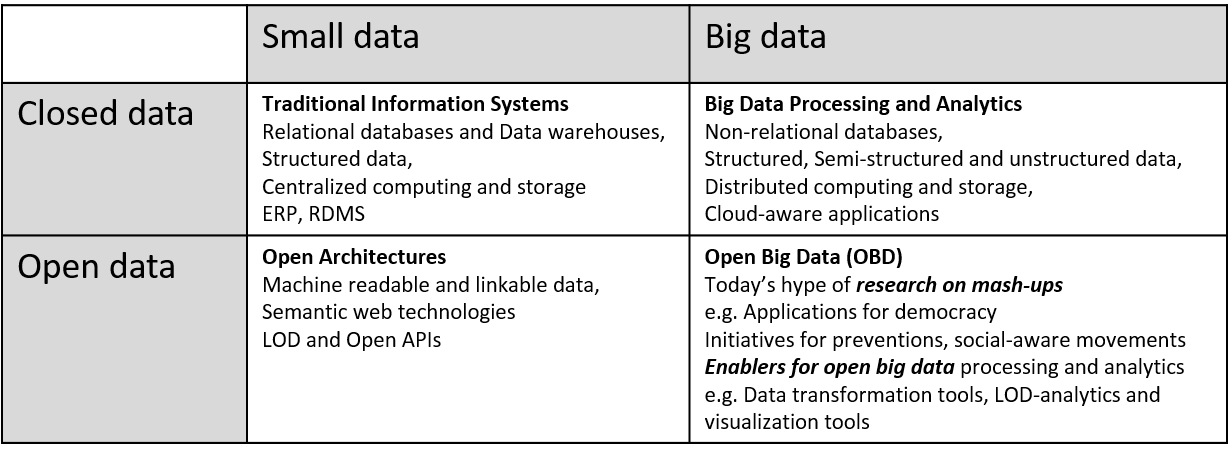
\includegraphics[width=38em]{./Figures/openbigdata}
	\begin{table}[htbp]
    \caption{Comparison on Open data and Big data \cite{reframingopenbigdata}}
    \label{tab:1}
	\end{table}
\end{center}
\noindent Table \ref{tab:1} compared the usage, formats  of open and big data and the systems or methods used to process them IS industry. Though, open data is not necessarily big, any new initiatives considering to support open data management should consider a scalable or workload-aware solutions to be proficient. 

\subsection{Linked Data and RDF Format}
\noindent Linked data provides a way to publish data on the Web in a distributed manner and using an interoperable and machine-readable format \cite{linkeddatasofar}. The data semantically described in machine understandable format and interlinked. In simple terms, linked data is data that is connected to other data using typed links coming from different sources.  Linked data relies on formulating data in Resource Description Framework (RDF) format \cite{rdfdefinition}. 
 
\noindent \textbf{RDF Format} : RDF represents a data with a generic \textit{graph-based data model} \cite{linkeddatasofar}, with which to structure data and describe it. The basic RDF data model represents a data in the form of subject, predicate, object which is usually called as \textit{triple}. A predicate mentions the relationship between subject and object. Set of triples form a RDF graph. RDF triple can contain\textit{ International Resource Identifiers} (IRIs) which is an extension of Universal Resource Identifier (URI) , \textit{blank nodes} which are disjoint from IRIs and literals  and \textit{literals} which has values such as string, numbers and dates. IRIs, blank-nodes and literals are distinct and distinguishable.  RDF vocabulary is a collection of IRIs. By engaging URIs using IRIs to identify resources, RDF to represent data resources and HTTP protocol as retrieval mechanism, linked data integrates well in the general architecture of Web which contains layers of linked documents that contains data. 

\subsection{Linked Data Preparation}
\label{sec:opendatapreparation}
\noindent Before publishing open data it is important that the data being published are complete, self contained, and can be used by anyone. To date, open data which are published are extracted from legacy databases, or from static logs, mostly \cite{collaborativeopendataversioning} in "silo formats" such as CSV, TSV, *SV, Excel formats ( XLS and XLSX ), JSON, XML, PDF. These data are typically "messy" (with errors, missing values, and consistencies) and cannot be immediately transformed into RDF format. Thus data cleaning is important aspect of linked data preparation. Linked data preparation has two main sub-processes - open data transformation and RDF generation. The usual process of creation of linked-data consists of raw data cleaning, transformation (mostly from tabular formats), mapping to one or more RDF ontologies and generating a semantic RDF graph \cite{datagraftsimplyfyingopendatapublishing}. 
\begin{center}
	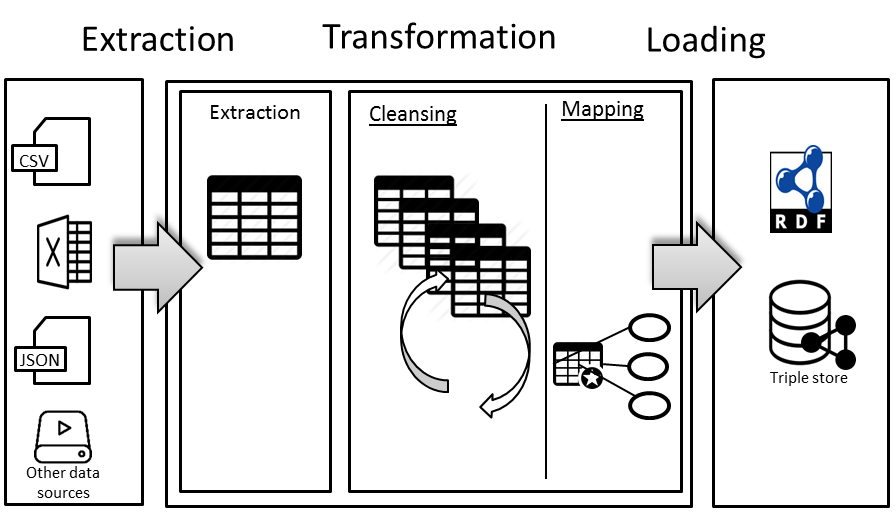
\includegraphics[width=38em]{./Figures/opendatapreparation2}
	\begin{figure}[htbp]
    \caption{Data cleaning in different data treatment techniques performed as expected}
    \label{fig:opendataprep}
	\end{figure}
\end{center}
\noindent Figure \ref{fig:opendataprep} shows this typical process of open data preparation. This process also can be compared/mapped to the well known Extract, Transform and Loading (ETL) operations \cite{collaborativeopendataversioning}. The major categories of cleansing and transformation operations are 
\begin{enumerate}
\item Analysis: Data analysis, statistical evaluation and data mining algorithms
\item Profiling: Identify and solve data quality problems (e.g. Misspellings, Cryptic values and abbreviations, Misfiled values and Word transposition) \cite{datacleaningprobsandapproaches}
\item Transformation: Operations to modify the data to fit the target schema (e.g. Embedded value,  Duplicate records, Pivoting and Un-pivoting, Slowly Changing Dimensions (SCD), Surrogate keys) \cite{datacleaningprobsandapproaches}\cite{ETL}
\item Cleaning: Detecting, removing and correcting dirty data together with schema-related transformation based on comprehensive meta-data (e.g. String problems) \cite{datacleaningprobsandapproaches}
\item Duplicate elimination: Identifying and merging duplicate records (e.g. Full duplicates and grouped duplicates)
\item Enrichment: Using additional information to improve data quality (e.g. Surrogate keys, SCD) \cite{ETL}
\end{enumerate}
\noindent These are typically needed in most data analysis tools. For the purpose of this thesis, we do not consider analysis since analysis are performed on top of integrated RDF data. The rest of the five categories are mostly used to help user to create a 'fit for purpose' data from messy data. 
\subsection{Data ingestion techniques}
Data ingestion technique is a data processing model or the routine how the input data is initially received and represented to be processed. The most frequently used data ingestion or treatment techniques in big data paradigm are batch processing, stream processing and micro-batch processing \cite{dataflow}. 
\begin{itemize}
\item \textbf{Batch processing} : Batch processing is a technique of treating the input data as a collection of data where the input data is assumed as fully available to be processed \cite{Sims-387}.
\item \textbf{Stream processing} :  Stream processing is a data processing model where data is treated as streams of data \cite{beyondbatchprocessing}. For example, a data stream can be generated based on event-by-event or complex-event-streams.
\item \textbf{Micro-batch processing} : Micro-batch processing is a combined version of batch processing and stream processing, which is to treat data as sequence of small batches of streams. Streams can be delayed to collect small batches or batch inputs can be split into small set of streams to become micro-batches. 
\end{itemize}
\subsection{Parallel computing and Parallel programming model}
Parallel computing is a type of computation where multiple computations performed simultaneously to increase application's performance \cite{parallelprg} . Parallel computing is more prevalent in the domain of multi-core-architecture (a system with multiple processing cores) . 
\begin{itemize}
\item \textbf{Parallel programming mode}l : Parallel programming model (PPM) consists an abstract parallel machine with its basic operations including arithmetic operations, spawning tasks, reading from and writing to shared memory etc \cite{PPM}. A PPM at least consists a memory model that describes how and when memory can become visible to different parts of the parallel computer. It is often associated with one or more parallel programming languages and libraries that realize this model.
\end{itemize}

\section{Research Problem}
\label{sec:problem}
 \noindent The necessity to publish open data has encouraged many governments, NGOs, NPOs and private institutions to publish their data. Nevertheless, the published data remains of low value since it is less useful without the prescribed interoperability. Statistics says that 80\% of data in publicdata.eu that aggregates data from 30 European data portals, are in\textit{ tabular formats} (Excel sheets or CSV files) \cite{nemreport}, which are considered \textit{silos}. In addition only 1\% of published data use vocabularies and are presented in RDF format \cite{nemreport}. Next generation research questions can only be answered only by integrating data from different sources \cite{nemreport}. This leaves the underlying goal of open data movement unsettled. Especially, how large open data silos can be processed to provide liquid data is unresolved. Data preparation of open big data  becomes the "\textit{enabler}" of active open data analysis, which implies easy data transformation from legacy data to liquid format. 

Due to its popularity in the data-domain, there are few initiatives who how tried to provide solutions towards achieving the goal of open data movement. However, they did not meet some of the crucial requirements that are essential and should be collectively provided, by an effective solution in growing open data era. We discuss the most important problems that are not solved by currently available systems and prioritized to be solved to provide a complete, long-lasting solution. 

\subsection{Lack of Scalability}
\noindent As we mentioned earlier open data can vary according to the data volume. An interview study reports that 31 of the 35 cleaning and analytic packages, tools or algorithms used in enterprises, are not scalable with the size of data sets \cite{2012-enterprise-analysis-interviews}. The system must be able to scale with the size of data, addressing both perceptional and computational limitations \cite{2012-enterprise-analysis-interviews}. Currently, the available data cleaning solutions, such as  OpenRefine \cite{openrefine}  and Wrangler \cite{2011-wrangler} are desktop applications, which cannot process large volumes of data. Furthermore, they require a large amount of dedicated local computing resources which prevents any other applications to be perform well on hosted system and prevents from efficient utilization of allocated resources. This highlights the need for a scalable, distributed solution of open data preparation. 
\subsection{Necessity of user-friendly and interactive data cleaning}
\noindent 
Open data workers are not typically technically oriented. In practice, open data workers are rather \textit{knowledge workers} who produce information from data - for example, researchers, data scientist,business analyst, medical workers and public administrators etc. Data workers report spending more than 80\% of their development time in data cleaning \cite{visualizationsandtransformationsinwrangling}\cite{Wisteria}\cite{journals/corr/KrishnanW0FG16}.

A data worker must be able to review and refine the cleaning process seamlessly. Visual analytic research \cite{Keim08visualanalytics:} suggests that tight visual interaction with user helps to remove errors easily and quickly. Specifically, visualization of data helps to immediately eliminate missing values, inconsistencies and wipe-out outliers \cite{visualizationsandtransformationsinwrangling}. An appropriate interface should be available to represent data and render immediate transformation results. This enables a self-serviced data preparation process and improves the accuracy of data preparation \cite{journals/corr/KrishnanW0FG16}. 

Often data preparation requires writing idiosyncratic scripts like Python, Scala, Perl and R or manual editing. This discourages a large number of workers from working with data, because they spend most of their time dealing with data, rather than excelling in their specialized domain \cite{visualizationsandtransformationsinwrangling}. Therefore, a user-friendly solution is crucial to allow the relevant end-user groups to do data analysis smoothly.
% Provided that open data workers are not usually technical oriented, performing data cleaning transformations must be easy and interactive, without needing technical knowledge. Many data cleaning solutions available today such as Wrangler, OpenRefine, KARMA require user to manually write domain specific scripts to create data cleaning transformations, that restricts the scope of users. This suggests that, using an automated, self-contained user interface that create transformation pipeline according to user inputs, to build cleaning transformations than manually writing scripts, will help to engage boarder-audience to actively perform data transformation.

\subsection{Inefficient processing of iterative data cleaning}
\noindent The cleanness or quality of data is difficult to determine before processing the data. Thus, the correctness and effectiveness of a data transformation work-flow should be verified by executing over sample data and improving the workflow if necessary, before applying it on the complete data. 

Data cleaning can bring new quality issues  while being cleaned. Such issues are referred to as \textit{nested-discrepancies },\cite{journals/corr/KrishnanW0FG16} and can be found only after certain cleaning have been done. Thus, data cleaning is an iterative procedure \cite{Wisteria} and should be repeatedly applied on incrementally updated data to provide accurate result. We, refer it as "incrementally iterative data cleaning". Hence, the data processing mechanism should be tolerant to iterative processing of large volumes of data. Some important aspects of interoperability in the data cleaning process are related to handling \textit{trail and error} scenarios, where an inappropriate data cleaning step should be able to rolled-back from data transformation process \cite{visualizationsandtransformationsinwrangling}. Currently, available systems don't perform efficiently during such iterative data cleaning. They reserve large amount of computing resources due to traditional underlined architecture

\subsubsection{Legacy architectural approaches result less useful}
\noindent Interactive data transformation implies the need for responsive user interfaces. Currently, this is possible only when data being processed is small since, the architectures of currently available systems were not designed with explicit consideration of processing large volumes of data. Traditional architectural approaches such as centralized processing (single threaded processes),  repetitive processing of complete input data, lack of load balancing, lack of optimization in handling redundant operations. When applications built using these approaches are used to process large volumes of data, it leads to poor-performance and/or non-functional systems. Proposed solution should be approached with large-scale application architectural concepts in mind, in addition to scalability.

\subsection{Lack of end-to-end data preparation solution}
\noindent The major problem that is widely faced in open data preparation is that there is no complete solution for open data preparations. Existing systems address only a part of needs, which result in manual data preparation using separate applications. This forces users to export and load data in several rounds. The existing solutions focus mainly on subsets of problem. KARMA \cite{karma}, LinDa project tools\footnote{http://linda-project.eu/} focuses mainly on formulating linked data from tabular formats whereas many other leading commercial tools such as IBM DataWorks\footnote{http://www.ibm.com/analytics/us/en/technology/cloud-data-services/dataworks/} , Talend Open Studio\footnote{https://www.talend.com/products/talend-open-studio} and Pentaho Kettel\footnote{http://wiki.pentaho.com/} are focusing mainly on data cleaning processes. KARMA provides basic facilities to do data cleaning. However, these data cleaning solutions lack some of the open data cleaning capabilities discussed in Section \ref{sec:opendatapreparation}. The main impediment to provide both solutions together can be the \textit{ lack of data abstraction that can work with tabular format and can be transformed into a graph-based model} to create RDF formats. A single solution should be available to perform data cleaning and transformation to RDF format seamlessly. 
\subsection{Availability and Accessibility}
\noindent Data preparation is not an instant process. A user should be able to perform consecutive transformations on a system for longer duration. In addition, in open data field, crowd-sourced data cleaning and transformation is getting popular which are called \textit{Multi-sector planning and analysis} \cite{multisectoranalysis}. It requires collaborative transformations, i.e. a data cleaning and transformation done by multiple partners. Pure offline applications hinders collaborative transformations. Cloud computing and distributed computing paradigm has proven solutions for availability issues. Providing solutions as a service enables more availability and waives complex environment installations and maintenance costs. This emphasis the need of an online data preparation application that can be shared-accessed and available between group of people.
\section{Research Motivation}
Due to the hype of big-data, there are ample of steps made towards meeting cutting-edge requirements of large-scale-processing. Advent of these striking technologies proven to be effective to process large volumes of data in real-time, serves as the basic motivation of this thesis, as they can be utilized to solve the unresolved problems faced in open data sector. We discuss the most associated topics that relies as the most important foundation of this thesis. Further, we also discuss the basics of relevant topics to support the important decisions made and to fill the knowledge-gap in the content. 

\textbf{Distributed-Data-Parallelization}

Distributed computing implies the programs that performs an operation by contacting other address spaces, possibly with other machines \cite{DistributedComputing}. Distributed data parallelizing is the most widely used computation model in big data that provides load balancing, fault tolerance of input data  \cite{Jackson2015517} and scalability, which performs a parallel computation by sharing partitioned data among distributed machines. MapReduce is the pioneer of distributed data parallization techniques. It is a programming model proposed by Google. By providing two primary parallel methods over distributed data (map and reduce) it achieves load balancing fault tolerance. However, MapReduce was later identified for its draw-backs on having huge file Input/Output (I/O) to store and load intermediate data. It is extremely slow and resource consuming when iterative operations are executed as pipeline of operations.
Figure \ref{fig:hadoop-high-io} shows how iterative jobs result in high I/O in MapReduce, since every stage is going through dish write and read. Further, Reduce operation can be only started only after all map jobs are completed.
\begin{center}
	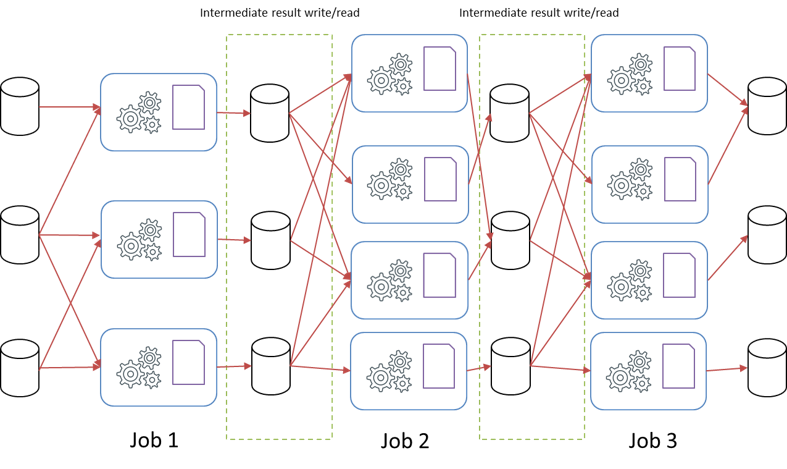
\includegraphics[width=32em]{./Figures/hadoop-high-io}
	\begin{figure}[htbp]
    \caption{High Input/Output behavior when iterative jobs performed on MapReduce}
    \label{fig:hadoop-high-io}
	\end{figure}
\end{center}
This leads to a long execution time. 
Hence, it doesn't suit to perform iterative operations as a pipeline and it is not a near-real-time responsive programming model. 
% Apache Hadoop\footnote{http://hadoop.apache.org/} is an open source implementation of MapReduce, which was a game changer in big data domain. Apache Hadoop also provided important distributed programming components such as  Hasoop Distributed File System (HDFS) and YARN Resource Manager. 
\subsection{In-memory computation}
In-memory computation, is the widely accepted programming model to process large files, in interactive and iterative processing. In-memory computation is performed on top of a Distributed Shared Memory (DSM) which holds read-only representation of data object in memory, that is created using memory distributed across a set of machines. The DSM is fault tolerant \cite{RDD}, and performs an operation by communicating with other parts of shared memory. This eliminates the drawback of having high I/O by holding the large-data on a DSM and not storing and loading back intermediate results of every iteration as depicted in Figure \ref{fig:in-memory-computing}.
 \begin{center}
	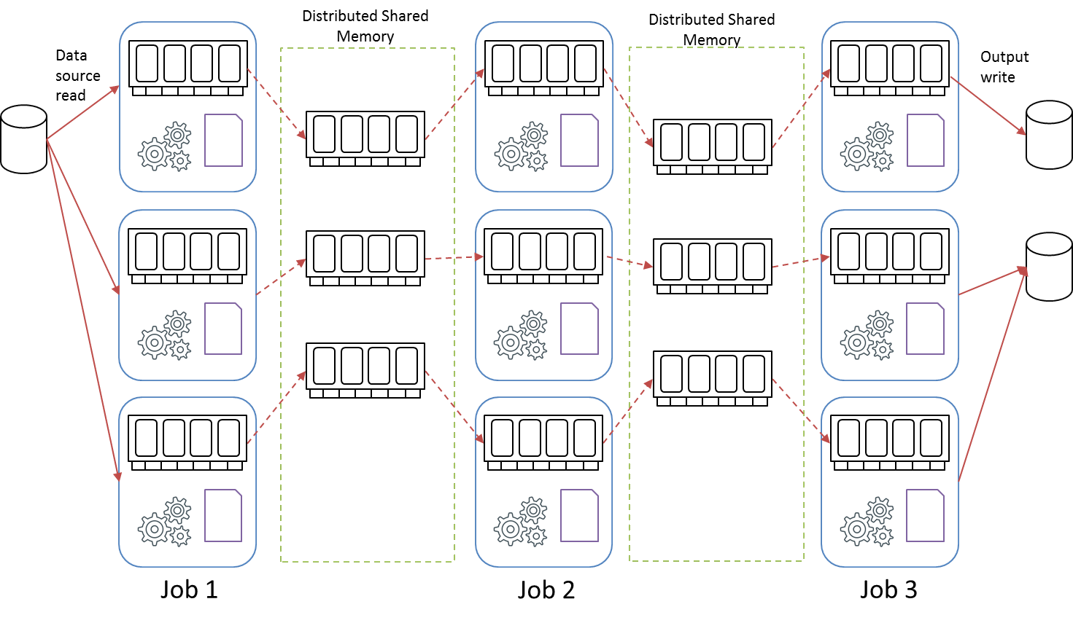
\includegraphics[width=32em]{./Figures/in-memory-computing}
	\begin{figure}[htbp]
    \caption{Behavior of in-memory-computing with iterative jobs}
    \label{fig:in-memory-computing}
	\end{figure}
\end{center} 
In-memory computing is realized by an open sourced implementation called Apache Spark. Apache Spark\footnote{http://spark.apache.org/} is today's "de-facto" of big data, a general purpose distributed data processing framework, which is built to meet recent big data requirements such as iterative jobs and interactive analysis \cite{Spark}. Spark realizes \textit{in-memory cluster computing} \cite{RDD} , using its main abstraction called \textit{resilient distributed dataset}.
Spark is claimed to be 10x - 100x faster than Hadoop (an implementation of MapReduce programming model) in iterative applications \cite{Spark}\cite{RDD}\citep{clashoftitians}\cite{Spark-improvements}, by benefiting from Spark's programming model. Spark also provides distributed cache and shared variables to reuse computed resources that suits iterative computation. 
\subsection{DataGraft}
\noindent \textit{DataGraft: One-stop-shop for open data management} \cite{onestopshotforopendata}  is a unique cloud-based solution for data transformation, integration and sharing. DataGraft is the only solution which supports open data preparation with both data cleaning and RDF transformation in a single package, as well as other relevant capabilities such as data hosting, querying and visualization. DataGraft responds to some of the most important challenges such as supporting repeatable and reusable cleaning, interactive data cleaning, real-time responsiveness, availability and accessibility, and general purpose open data preparation support. DataGraft integrates \textit{Grafterizer}\footnote{https://github.com/dapaas/grafterizer}, an interactive open data preparation tool, which currently uses Graftwerk for data transformation purpose. Graftwerk is a Web Service that has a sandbox which executes transformation pipeline built using a data transformation library called Grafter\footnote{http://grafter.org/} that uses traditional data processing techniques for data cleaning and RDF transformation called . This traditional, centralized processing on a single hosted system, obstructs scalability. As DataGraft is facing larger volumes and more complex clean-up and transformation problems, it is essential to introduce parallelism, scalability and an optimized process. 

In this thesis, we respond to the latest challenges and demands of open data preparation by remodeling the interactive data preparation tool of \textit{DataGraft}\footnote{https://datagraft.net/} project to met the problems mentioned in Section \ref{sec:problem} using in-memory-computing approaches.
% \section{Summary change}
% \label{sec:researchproblem}
% The open data paradigm is expanding, and has enjoyed interest from governments, independent researchers, NGOS, NPOs and private business organizations who are moving towards transparently distributing their data. However, there is an \textit{absence of a complete efficient and effective open data preparation solution}. Firstly, there is a lack of an efficient, scalable data cleaning solution of "messy" data. Secondly, there is no simplified soluti\on that provides both data cleaning and RDF transformation that can be used by non-technical users. Further, there is a gap in reanalyzing latest requirements in the domain that are essential to be solved to create a general purpose system. In summary, there is a need for a general purpose system that should be automated, user friendly and immediately effective. Having a service-based solution is essential to eliminate complex installation and maintenance process as non-technical users are also targeted to be benefited from this system. The main goal of this research is to design and implement a solution that meets all of the aforementioned requirements. 
objective
find suitable data ingestion n utilize in-mem comp to provide solu that can meet those req
\section{Research Questions}
\label{sec:reseach-ques}
\noindent The problem addressed by this thesis spreads across different key topics. These can be formulated into the following research questions:
\begin{enumerate}
\item Which is the most suitable data ingestion technique (batch, micro-batch and continuous-flow) and level of responsiveness  (real-time, near real-time and off-line batch-jobs) that satisfy the requirements of interactive data cleaning and transformation?
% \item Which is the most appropriate programming model, between MapReduce (Hadoop), LINQ (Dryad), RDD (Spark), to support chosen data treatment technique ensuring the efficiency and effectiveness of iterative data clean-up operations that can scale with respect to data volume?
\item how distributed-data-parallelization and in-memory computing can be utilized to provide data prepratation solution that is scalable, interactive, responsive in real-time, and available as a service?
% \item How to provide an appropriate underlying distributed data abstraction that can be used both to process tabular data, and to ultimately produce graph data? How can such a data abstraction be re-purposed to support the required data cleaning and RDF transformation capabilities?
% \item How to re-engineer the operation of an interactive transformation engine efficiently implementing the open data preparation features using identified data abstraction?
\end{enumerate}

\section{Research Methodology}
The research methodology followed for this research duly relies on design science \cite{von2004design} research following the guidelines for Information Systems (IS) research. The research problem and proposed solution artifact are derived from a literature survey. The literature survey consists of publications, scientific journals, technical reports and also analysis of widely used tools due to gap of studies carried out on latest solutions. The solution for Research question 2 from Section \ref{sec:reseach-ques} will be derived from analyzing literature survey in the relevant context. The solution consists analytic results, implementation by extension, adaptation, integration and remodeling.  By following design science guidelines, the solution will be evaluated using qualitative analysis method. Furthermore, the research and end results assure the  required research relevance, contributions, scientific rigor and design as a search process. 
\subsection{Work plan}
\noindent With respect to the discussions in Section \ref{sec:opendatapreparation}  and \ref{sec:problem}, we define the initial construct for the research as: 1) identifying suitable constructs that answers the research questions, and  2) an implementation of a minimum viable product (MVP) that consists of proving integrated interactive scalable support for data cleaning in accordance to the discussions above with a proof-of-concept (POC) scalable abstraction for RDF transformations that implements scalability and performance improvements. The research approach and end-artifact should be open-source and continuously evolving.  The work plan is decided accordingly consists bellow steps:
\begin{enumerate}
\item Analyze the state of the art techniques of large-scale-data-processing techniques that can be used to implement iterative large scale processing and identify one that suits the most?
\item Analyze the state of the art supporting technologies, frameworks and tools providing identified technique, and determine how feasible, viable and popular they? Choose the most suited tool
\item Conduct a feasibility study of implementing MVP using the chosen tool.
\item Identify the limitations and assumptions of planned work. 
\item Implement MVP including extensions of chosen tools, adaptations to domain-specific requirements, and integration with existing system components.
\item Evaluate the MVP against existing implementations.
\item Document the research contributions. 
\end{enumerate}

The rest of the thesis is organized as follows. In Chapter \ref{Chapter2} , contemporary requirements of an interactive, scalable open data preparation are derived from literature review. Further, related works that has been done in the domain of this thesis are analyzed. Chapter \ref{Chapter3}, we analyze the relevant state-of-the-art techniques and technologies to identify the core elements to design our solution. In Chapter \ref{Chapter4}, we describe the design and implementation of the proposed solution. In Chapter \ref{Chapter5}  we provide the evaluation of implemented prototype. Finally, in Chapter \ref{Chapter6}, we conclude our results and contributions and define the future works that can be carried out and relate to this work. 

% Other requirement.
% Transformation Mapping functions should be declarative and should be reusable for other data.especially a workflow transformation structure  should be supported execute all data transformation steps for multiple sources. Schema level transformation and cleaning should be specified by declarative query and mapping language as far as possible, to enable automatic generation of the transformation code. It should be possible to invoke user-written cleaning code and special purpose tools during a data transformation workflow.  transformation steps may request user feedback . auto duplicate elimination and schema matching.
% Verification: The correctness and effectiveness of a transformation workflow and the transformation definitions should be tested and evaluated, e.g., on a sample or copy of the source data, to improve the definitions if necessary
% more work is needed on the design and implementation of the best language approach for supporting both schema and data transformations.operators such as Match, Merge or Mapping Composition have either been studied at the instance (data) or schema (metadata) level 

% Most of the data transformation tools don't have clear separation of logical specification of data transformation and physical implementation. \cite{declarativedatacleaning}
% todo: current systems support limited data cleaning support focusing on transformation and schema translation. should provide more support to data cleaning. data must be extracted from multiple sources and transformed n combined  during query time.  

% Why better than existing ETL tools? in usual ETL workflows transformations are mentioned in high-level-language. Logical query optimization is not possible unless the user designs it with consideration upfront\cite{ETL}. Lot of work for designer. Now spark catalyse code generator transforms pipe into optimized logical queries. 

% Questions: Can we use espemino as sample and ask them to give bigger data? 
% The dataset used to show in uio seminar by titi
% As the need for open data sharing is increasing, there are some  initiatives that try  solve these needs. However, such initiatives only address a subset of needs such as either data cleaning or transformation (or any other combinations of the activities in the data sharing process\textbf{ confusing??/)}.  In this thesis, we explore how can we provide a scalable open data sharing needs as a service by eliminating current limitations. 


% \section{Research Motivation}

% a comparative study on leading solution providers

% Definitions  
% Open data 

% Linked data 

% Data tranformation in open data : combination of data cleanging and transformation it to RDF

% Data cleaning 
% Scalable

% Near real time 
% Interactive transformation 

% Linked Data
% Open data is commonly shared in Linked Data format, which is defined as a set of best practices for publishing and connecting structured data on the web\cite{linkeddatasofar}.  Open governments, public administrations and other commercial organizations have recently started publishing large amount of structured data. There 

% Open data is the data that can be used, re-used and redistributed by anyone without any limitations or at minimal limitations\cite{opendatahandbook}. 


% %----------------------------------------------------------------------------------------

% \section{Research Motivation}

% In this section we outline several reasons how the research presented in this paper  addresses important concerns of 
% related work 
% explain the archi
% open refine
% karma
% trifacta
% ibm dataworks
% talent 
% lightweight transformation of tabular open data to rdf
% similar solutions address the domain and what they lack and how they are related to our work


% \subsection{Background}

% \noindent As we mentioned earlier, important challenges during 

% %----------------------------------------------------------------------------------------

% \subsection{Motivating Scenario}
% DataGraft.net, a cloud based open data sharing platform tries to address all these needs together as a service. However, it has limitations of transforming large data.
% \noindent To have a better understanding of the previously discussed challenges and approaches, the following motivating scenario has been developed: 
% introduce datagraft in detail, how it address the common needs in big picture. 
% architecture
% todays limitations in data transformation.


% %----------------------------------------------------------------------------------------

% \subsection{Discussion}
% \label{sec:Discussion}
% why this limitation
% who eliminating this can help 
% what is expected from this?

% %----------------------------------------------------------------------------------------

% \section{Research Problem}

% \noindent In this work we focus on two challenges: (i) combination of the declarative and imperative approaches to the application provisioning and deployment, and (ii) continuous deployment of cloud applications. Based on this, the research problem may be formulated as follows: 

% How to transform larger data without technical knowledge
% how interactive transformation of large files can be done in near-real-time?

% \begin{center}
% "How can we enable both, flexibility and fine-grained control, in the deployment and provisioning of multi-cloud applications, and allow efficient run-time management of such applications?"
% \end{center}

% \section{Research Questions} 

% \noindent The problem addressed by this thesis rises the following questions:

% \begin{enumerate}
% \item  How imperative and declarative approaches can be combined? Does a combined approach furnish a more efficient and flexible solution?

% \item  How to create a DSL for the specification of deployment plans that can be used in combination with declarative deployment topology models, and programmatically by a third party?

% \item  How such DSL could be used to support efficient continuous deployment of multi-cloud applications?

% \end{enumerate}

% %----------------------------------------------------------------------------------------

% \section{Research Methodology}
% In this section we explain our research methodology and develop a research work plan.

% %----------------------------------------------------------------------------------------
% \subsection{Methodology}

% \noindent The adopted methodology of this thesis relies on a literature survey and design science \cite{von2004design}. Literature survey covers not only publications in scientific journals but also analysis of widely used tools because provisioning and deployment processes relate more to the practical side of computer science than its theoretical underpinnings. Design science guidelines help us in the development of our solution and ensuring that our results are relevant, verifiable and appropriately evaluated.

% %----------------------------------------------------------------------------------------
% \subsection{Work Plan}
% Following the discussion from the Section \ref{sec:Discussion} and, according to the research problem, we can define the initial set up for the research: the approach that we will work on must be declarative, open source and provide support for the continuous deployment. Then, the work plan to answer research questions includes the following steps:

% \begin{enumerate}
% \item  Analyze state of the art tools and approaches for 

% \item  Choose a declarative approach for the improvement.

% \item  Analyze how deployments plans are defined in imperative approaches. Extract common characteristics and limitations of languages used to define deployment plans, and create a domain-specific workflow definition language to specify such plans.

% \item  Integrate a chosen approach, including the continuous deployment functionality, with created DSL.

% \end{enumerate}

% \noindent The rest of the thesis is organized as follows. In Chapter 

% solution analysis - state of the art spark
% Dataframe 
% feasibility test
% dataframe performace tests
% https://databricks.com/blog/2015/02/17/introducing-dataframes-in-spark-for-large-scale-data-science.html

% https://0x0fff.com/spark-dataframes-are-faster-arent-they/

% implementation - Scalable transformation of open data

% problem
% archi- should explain clearly for backend n front-end 
% solution components
% sparker
% scalable-graftwerk
% grafterizer
% deployment - possible on local and cluster 

% evaluation

% Integration n usability

% functional coverage- how much persisted from earlier, how much can be added newly
% consistency-
% reliability - no sandbox
% scalability
% availability

% Performance evaluation

% experiment setup

% of single machine - oldgraftwerk , sparker on local, open refine

% for different file size, same pipeline

% trifacta, open refine, setup on cluster

% conclusions
% posible transformation for big data. without limitation. can be hosted in local cluster is provided service is not enough. the limitation is eliminated. 
% technical contributions
% scientific contributions

% appendix


%----------------------------------------------------------------------------------------